\Echapter{Plotting Group FEAT Results Against Behavioral Measures}{Melissa A. Reilly}{mreilly@uw.edu}
\label{sec:groupfeatreport}
In neuroimaging research it is often beneficial to examine your results in conjunction with behavioral data to gain a more complete understanding of your effect. For example, it is certainly informative enough to look at group activations from subjects completing a memory task within the scanner; however, taking it a step further and examining the relationship of subjects' accuracy scores on the task to activation arguably paints a richer picture. 

The example provided here does exactly this using a subset of a dataset from OpenFMRI.org (\url{https://openfmri.org/dataset/ds000115}). These study subjects completed a working memory task (the n-back) within the scanner and their accuracy scores were tracked. In this example, we will visualize each significant cluster, identify it, and plot activation within the cluster against the accuracy scores. 

The code for this example is in \texttt{\$MAKEPIPELINES/WorkingMemory}. If you are not at IBIC, from within that directory, call the \texttt{PrepareExample} script to download the data and organize the directory. Note that this script may take upwards of 30 minutes depending on your machine. This script will create subject directories for 31 subjects. In your command line, you can type: 
\bashcmd{bash PrepareExample}

Once the download is complete, you can use the \texttt{prepare} target to run the lower-level FEATs.
\bashcmd{make -f makefiles/Makefile -k -j TARGET=prepare}

When the lower-level FEATs have completed, you can run the higher-level group analysis. A design file is already prepared for this:
\bashcmd{Feat lib/GROUP_2BACK.fsf}

If you open the file with \texttt{Feat}, you will note that the accuracy scores are already included (these scores were obtained from \texttt{data/demographics.txt}). You should check that the paths to the input files and standard brain are correct on your system. Once you have verified that they are, click "Go" to run the analysis. 

This example uses two separate Makefiles in three steps to create the final product. The first step is to read the results from the \texttt{.gfeat} directory to generate masks for each significant cluster. This is done with \texttt{makefiles/Makefile.gfeat}. The second step is to use an FSL tool (\texttt{featquery}) to warp each mask into the subject's space and extract from it the mean z-score. This is done with \texttt{makefiles/Makefile.subdir}. The final step is to use \texttt{makefiles/Makefile.gfeat} to create a spreadsheet within the \texttt{.gfeat} directory containing all the \texttt{featquery} z-scores, plot all those values against n-back performance, and create an HTML report containing the plots as well as visualization of the clusters. We will begin with \texttt{makefiles/Makefile.gfeat}:

\begin{lstlisting}
	SHELL=/bin/bash
	export SHELL
	
	FSL_DIR=/usr/share/fsl/5.0
	
	ifeq "$(origin MAKEPIPELINES)" "undefined"
	MAKEPIPELINES=/project_space/makepipelines
	endif
	HOMEDIR=$(MAKEPIPELINES)/WorkingMemory
	GF=$(basename $(shell basename %*\`{}*pwd%*\`{}*))
	%*\lnote*ALLCOPES=$(wildcard cope*.feat) 
	NUMMASKS=%*\`{}*ls MASKS | wc -l%*\`{}*
	
	%*\lnote*group1: .readyforfq
	group2: FQresults_allSUBS FQresults_EVs $(MASKLIST:%=FQresults_%) FQresults_DATA
	group3: rplots $(MASKLIST:%=PLOTS/%_brain.png) $(CLUSTLIST:%=AQUERY/%) FQreport.html
	
	.PHONY: group1 group2 plots group3 clean.gfeat 
	
	clean.gfeat:
		rm -rf .readyforfq FQ* design2.mat sed* PLOTS MASKS CLUSTERS AQUERY
\end{lstlisting}
As you've seen before, we define our \texttt{SHELL} and \texttt{FSL_DIR} variables for consistency, and specify the location of the project directory (\texttt{HOMEDIR}). We also include a "clean" function to remove any of the outputs generated from the \texttt{Makefile.gfeat} makefile. To accommodate the back-and-forth previously mentioned, \texttt{Makefile.gfeat} is run in several small chunks, so the  \texttt{makefile} is divided into three phony targets (\texttt{group1}, \texttt{group2}, and \texttt{group3}) to make it easier to run from the command line. Note that if you are looking at the code in the actual makefile, you will find that the two chunks of code defining variables for \texttt{group2} and\texttt{group3} have not been included above -- do not fret; these will be explained further down the line in this documentation. 

After specifying the path to the FSL directory, we prepare some variables to help \maken{} complete the "group1" target, which creates the masks we need before we move into the subject directories. \lnum{1} The \texttt{ALLCOPES} variable uses a wildcard to obtain a list of all the \texttt{cope*.gfeat} subdirectories within the \texttt{.gfeat}. The \texttt{NUMMASKS} variable will list all the masks in our soon-to-be-created \texttt{MASKS/} subdirectory. \lnum{2} The "group1" target has only one prerequisite: \texttt{.readyforfq} :

\begin{lstlisting}

	.readyforfq:
		mkdir -p MASKS ;\
		mkdir -p CLUSTERS ;\
		
		%*\lnote*for COPE in $(ALLCOPES); do \
			%*\lnote*Zs=%*\`{}*ls $${COPE} | grep ^cluster_mask_zstat | wc -l%*\`{}* ;\
			WHICHZ=%*\`{}*seq 1 1 $${Zs}%*\`{}* ;\
			for CM in $${WHICHZ}; do \
			  %*\lnote*CNUM=%*\`{}*fslstats $${COPE}/cluster_mask_zstat$${CM}.nii.gz -R | awk `{ print $$2 }'%*\`{}* ;\
				for VAL in %*\`{}*seq -w 01 01 $${CNUM%%.*}%*\`{}*; do \
					$(FSL_DIR)/bin/fslmaths $${COPE}/cluster_mask_zstat$${CM}.nii.gz -thr $${VAL} -uthr $${VAL} -bin MASKS/$${COPE%.*}_z$${CM}_m$${VAL}.nii.gz ;\
					$(FSL_DIR)/bin/fslmaths $${COPE}/thresh_zstat$${CM}.nii.gz -mas MASKS/$${COPE%%.*}_z$${CM}_m$${VAL}.nii.gz CLUSTERS/$${COPE%.*}_z$${CM}_m$${VAL}.nii.gz ;\
				done ;\
			done ;\
		done ;\
		
		echo "$(NUMMASKS) masks found for $(GF)!";\
		touch .readyforfq
\end{lstlisting}

We begin by creating \texttt{MASKS/} and \texttt{CLUSTERS/} subdirectories to house the files we are about to create.  We have already defined our \texttt{ALLCOPES} variable to be anything in the directory that fits the \texttt{cope*.feat} wildcard. In this example we have five copes, which are defined in \texttt{GROUP_2BACK/design.fsf}, but a given analysis could have any number, so a wildcard allows the program to be accommodating to both simpler and more complex designs. \lnum{3} We want \maken{} to go into each of these copes, find out how many \texttt{cluster_mask_zstat*.nii.gz} images are in each ( \lnum{4}), and then how many unique clusters are in each of those ( \lnum{5}). Though not ideal as far aesthetics are concerned, some shell variables and looping is the simplest way to do this.  (It is worth pointing out that the double \texttt{\$\$} is intentional -- when referring to shell variables \maken{} requires that you escape the \texttt{\$} with another \texttt{\$}.) For each unique cluster, \texttt{fslmaths} will create a binary mask to be placed in the \texttt{MASKS/} directory, and will then use that mask to create a thresholded image in the \texttt{CLUSTERS/} directory. The images are identical, except that the \texttt{MASKS/} one is binarized, and both are named according to the same convention (cope(\#)z(\#)m(\#).nii.gz). To put all this into practice, move into \texttt{GROUP_2BACK.gfeat} and run the "group1" target (NOTE: the "group1" target should NOT be parallelized):
\bashcmd{make -f ../makefiles/Makefile.gfeat -k group1}

As the "group1" target completes, it will print the number of masks created to the terminal. If there are no masks, there is nothing left to do; this analysis has 13 masks, which you can confirm by looking in the \texttt{MASKS/} subdirectory. Return to the \texttt{WorkingMemory} directory. The next step is to pass these masks to \texttt{featquery} to run in the individual subject directories. Let us look at our next makefile, \texttt{makefiles/Makefile.subdir}:

\begin{lstlisting}
	SHELL=/bin/bash
	export SHELL
	
	ifeq "$(origin MAKEPIPELINES)" "undefined"
	MAKEPIPELINES=/project_space/makepipelines
	endif
	HOMEDIR=$(MAKEPIPELINES)/WorkingMemory
	
	SUB=$(shell pwd|egrep -o `sub[0-9][0-9][0-9]')
	SUBDIR=$(shell pwd)
	
	.PHONY: prepare clean.prepare clean.featqueries featqueries

	FSL_DIR=/usr/share/fsl/5.0
\end{lstlisting}

In the beginning of the file we define the variables we will need. We define our \texttt{HOMEDIR} and \texttt{FSL_DIR} the same as before. Because this part of the analysis will go into the individual subject directories, we define a \texttt{SUB} variable to indicate to \maken{} where to find our subjects' data. Finally, we declare our phony targets: "featqueries" and "clean.featqueries". You will notice "prepare" and "clean.prepare" targets being listed as PHONY as well; these targets, along with most of the middle of \texttt{Makefile.subdir}, pertains to the lower-level analyses we already ran. Therefore, we can skip to the bottom of the file below the line of \# signs:
\begin{lstlisting}	
	%*\lnote*GROUPDONE=$(shell if [ $(GF) ]; then echo true; else echo false; fi)
	ifeq ($(GROUPDONE), true)
	
	MASKLIST=$(basename $(basename $(shell ls $(HOMEDIR)/$(GF).gfeat/MASKS/)))
	
	featqueries: $(MASKLIST:%=$(SUBDIR)/$(SUB)_2BACK_firstlevel.feat/fq_$(GF)_%/report.txt)
	
	clean.featqueries:
		rm -rf $(SUBDIR)/$(SUB)_2BACK_firstlevel.feat/fq*
	
	%*\lnote*define query
	$(SUBDIR)/$(SUB)_2BACK_firstlevel.feat/fq_$(GF)_$(1)/report.txt: $(HOMEDIR)/$(GF).gfeat/.readyforfq
		if [ -d $(SUBDIR)/$(SUB)_2BACK_firstlevel.feat/fq_$(GF)_$(1) ]; then rm \
		-rf $(SUBDIR)/$(SUB)_2BACK_firstlevel.feat/fq_$(GF)_$(1); fi ;\
		$(FSL_DIR)/bin/featquery 1 $(SUBDIR)/$(SUB)_2BACK_firstlevel.feat 1 stats/zstat`echo $(1) | cut -c 5` fq_$(GF)_$(1) $(HOMEDIR)/$(GF).gfeat/MASKS/$(1).nii.gz ;\
		echo "%*\`{}*cat $(SUBDIR)/$(SUB)_2BACK_firstlevel.feat/fq_$(GF)_$(1)/report.txt | awk `{print $$$$6}'%*\`{}*" ;\
		
	endef
	
	%*\lnote*$(foreach mask,$(MASKLIST),$(eval $(call query,$(mask))))
	
	endif
\end{lstlisting}

\lnum{6}We define a \texttt{GROUPDONE} variable for two reasons: first, to run either the "featqueries" or "clean.featqueries" targets, the name of the group FEAT is necessary, so we don't want them to try to run unless \texttt{GF} is defined; second, it is entirely likely that a given project directory will have multiple group-level FEATs, so we want to ensure we are using the masks and featqueries unique to the one we want! The \texttt{MASKLIST} variable uses the \texttt{\$(GF)} variable provided at the command line to look at the \texttt{MASKS/} directory in that group FEAT and save the names without the \texttt{.nii.gz} extension. 

Because a given group FEAT can have any number of masks, it is imperative that our program is flexible enough to deal with a degree of uncertainty. We need to write a smarter recipe, where \maken{} will know to take each mask, run \texttt{featquery}, and create the output file -- and all this without us specifying how many masks or how they are named. \lnum{7} To do this, we define a function called \texttt{query}. The recipe defined within it is written like any other, but makes use of a \texttt{\$(1)} variable, an argument. \lnum{8}We use a combination of \maken{}'s \texttt{foreach}, \texttt{eval}, and \texttt{call} to read all the masks contained in \texttt{MASKLIST} and submit each of those as the argument to \texttt{query}. From the main project directory, run the "featqueries" target (and this time, parallelizing is encouraged!). When running the Makefile from the command line, be sure to include the \texttt{GF=GROUP_2BACK}, and note that the \texttt{.gfeat} extension should not be included:
\bashcmd{make -f makefiles/Makefile -k -j TARGET=featqueries GF=GROUP_2BACK}

When all the featqueries have completed, we return to \texttt{makefiles/Makefile.gfeat} to look at the "group2" variables:

\begin{lstlisting}
	INPUTS=%*\`{}*cat design.fsf | grep "set feat_files(" | awk `{print $$3}' | sed -e `s/"//g'%*\`{}*
	%*\lnote*INPUTShack=%*\`{}*cat design.fsf | grep "set feat_files(" | awk `{print $$$$3}' | sed -e `s/"//g'%*\`{}*
	INPUTNUM=%*\`{}*cat design.fsf | grep "set feat_files(" | wc -l%*\`{}*
	MASKLIST=$(basename $(basename $(shell ls $(HOMEDIR)/$(GF).gfeat/MASKS)))
	RESULTS=$(MASKLIST:%=FQresults_%)
\end{lstlisting}

There are only a few variables we need for completing the "group2" target, which compiles the spreadsheet containing the subject list, explanatory variables (EVs) and the mean values for each mask. We declare \texttt{INPUTS} to be our list of subject inputs, which we are reading from the \texttt{.gfeat}'s \texttt{design.fsf} file; \texttt{INPUTNUM} is simply a count of how many inputs we have. You will notice that \texttt{INPUTShack} is defined almost identically to \texttt{INPUTS}, with the exception of two additional \texttt{\$} in the \texttt{awk} command -- we'll come back to this. As in \texttt{makefiles/Makefile.subdir, MASKLIST} is a list of all the masks in the \texttt{MASKS/} subdirectory. The \texttt{RESULTS} variable contains a list of the titles of the results pages we will create, one for each mask, the names of which are obtained by pattern substitution of the \texttt{MASKLIST} variable. Recall from earlier that the "group2" target has four prerequisites: \texttt{FQresults_allSUBS, FQresults_EVs, \$(MASKLIST:\%=FQresults_\%), FQresults_DATA}, the last of which being the final output of this target:

\begin{lstlisting}	
	FQresults_DATA: .readyforfq FQresults_allSUBS FQresults_EVs $(RESULTS)
		paste -d',' FQresults_allSUBS FQresults_EVs $(RESULTS) > FQresults_DATA
\end{lstlisting}
\texttt{FQresults_DATA} will be a comma-separated spreadsheet that contains a column of the subject IDs, the names of the EVs and their values for each subject, and the names of the masks and the mean z-scores extracted from each of them for each subject. This file is created by pasting together several smaller files which are created below.

\begin{lstlisting}	
	FQresults_allSUBS: .readyforfq
		echo $(INPUTNUM)_SUBJECTS >> FQresults_allSUBS ;\
		echo $(INPUTS) >> FQresults_allSUBS ;\
		sed -i `s/ /\n/g' FQresults_allSUBS ;\
		rm -f sed*
\end{lstlisting}

\texttt{FQresults_allSUBS} is a text file containing each subject ID, and it will be the first column of the \texttt{FQresults_DATA} spreadsheet. We simply print "\texttt{\$(INPUTNUM)_SUBJECTS}" to the file to serve as the column header. We \texttt{echo} the subject IDs (the contents of \texttt{\$(INPUTS)}) after that, and use \texttt{sed} to replace spaces with linebreaks. 

\begin{lstlisting}
	FQresults_EVs: .readyforfq
		NUMEV=%*\`{}*cat design.mat | awk `/NumWaves/ {print $$2}'%*\`{}* ;\
		%*\lnote*for EV in %*\`{}*seq 1 1 $${NUMEV}%*\`{}*; do \
			echo -ne "%*\`{}*cat design.fsf | grep "set fmri(evtitle$${EV})" | awk `{print $$3}'%*\`{}*," >> FQresults_EVs ;\
		done ;\
		echo >> FQresults_EVs ;\
		%*\lnote*cat design.mat | tail -n $(INPUTNUM) >> design2.mat ;\
		NUMEV=%*\`{}*cat design.mat | awk `/NumWaves/ {print $$2}'%*\`{}* ;\
		%*\lnote*for c in %*\`{}*seq 1 1 $${NUMEV}%*\`{}*; do \
		 	while read line; do \
					SN=`echo $${line} | awk -v i="$${c}" '{print $$i}'` ;\
					EXP=`echo $${line} | awk -v i="$${c}" '{print $$i}' | awk -F 'e' '{print $$2}'` ;\
					BASE=`echo $${line} | awk -v i="$${c}" '{print $$i}' | awk -F 'e' '{print $$1}'` ;\
					%*\lnote*NUM=`echo "scale=1; $${BASE}*(10^$${EXP##*+}.0)" | bc` ;\
					echo "$${SN} ---> $${NUM}" ;\
					sed -i "s/$${SN}/$${NUM}/g" design2.mat ;\
			done < design2.mat ;\
		done ;\
		sed -i `s/\t/,/g' design2.mat ;\
		cat design2.mat >> FQresults_EVs ;\
		sed -i `s/,$$//g' FQresults_EVs ;\
		sed -i `s/\"//g' FQresults_EVs ;\
		rm -f sed*
\end{lstlisting}
\texttt{FQresults_EVs} is another text file that will make up the column(s) immediately to the right of the subject IDs in \texttt{FQresults_DATA}, with the number of columns being determined by how many EVs were included in your \texttt{.gfeat} model (in our case, two). This recipe reads the \texttt{.gfeat}'s \texttt{design.mat} and \texttt{design.fsf} files, which contain all the information we need. Our end goal is to have a column for each EV where the EV name is printed in the first row and the value for each subject is printed on the subsequent lines, with each column being separated from the next with a comma. The \texttt{NUMEV} variable will read the header of the \texttt{design.mat} file to determine the number of EVs. \lnum{10} We will then use a simple \texttt{for} loop to read the names of the EVs one through \texttt{\$(NUMEV)} from \texttt{design.fsf}, and print all those names to the first row of \texttt{FQresults_EVs}. To obtain the values for these EVs, we basically want the information contained in \texttt{design.mat}, but not all of it, and not in that format. We will copy the lines of \texttt{design.mat} that pertain to the individual subjects to \texttt{design2.mat} by using the \texttt{tail} command in conjunction with our \texttt{INPUTNUM} variable. 

In a perfect world, this is where this recipe would end; however, FEAT stores the values in \texttt{design.mat} in scientific notation. We cannot pass the numbers to R for graphing in scientific notation, so we will have to correct that formatting issue. \lnum{12} We again reference the \texttt{NUMEV} variable so we can move through the EVs column-by-column, and then use a \texttt{while read loop} to correct each value in that column. We use \texttt{awk} to capture the coefficient and exponent separately, and \lnum{13} then use \texttt{bc} to do the math and put the numbers in standard notation. A series of \texttt{sed} commands at the end of the recipe cleans up the data further: the first exchanges tabs for commas, the second removes commas at the end of a line, and the last removes quotes that \texttt{FEAT} puts around the values. \texttt{FQresults_EVs} is now ready to be pasted next to \texttt{FQresults_allSUBs} in the creation of \texttt{FQresults_DATA}; we need only the columns that correspond to the individual masks:
\begin{lstlisting}
	define getvalues
	
	FQresults_$(1): .readyforfq
		echo "$(1)" > temp_$(1) ;\
		for i in $(INPUTShack); do echo %*\`{}*cat $$$${i}/fq_$(GF)_$(1)/report.txt | awk `{print $$$$6}'%*\`{}* >> temp_$(1); done ;\
		mv temp_$(1) FQresults_$(1)
		
	endef
	
	%*\lnote*$(foreach mask,$(MASKLIST),$(eval $(call getvalues,$(mask))))
\end{lstlisting}
As you well know by now, a function is our best bet for dealing with the unpredictable nature of the number of masks in our analysis. The \texttt{getvalues} function will create a text file for each mask called "\texttt{FQresults_MaskName}", which will have the name of the mask in the first row and the values for each subject in subsequent rows. \lnum{14}As we did with the \texttt{query} function, we submit each mask name as an argument. We have already discussed that using shell variables requires an extra \texttt{\$}, but this gets even more complicated within a function. Additional escapes are necessary, hence the four \texttt{\$} preceding each shell variable.  \lnum{9}This is also the reason for needing the \texttt{INPUTShack} variation of the \texttt{INPUTS} variable - the \texttt{awk} command within it needs additional escapes to be used within \texttt{getvalues}. For each mask, the recipe looks into each subjects corresponding \texttt{featquery} results page, grabs the mean value, and prints it to the \texttt{FQresults} file for that mask.

Despite the lengthy explanation, this all runs very quickly. Move into the \texttt{GROUP_2BACK.gfeat} directory and run the "group2" target. You should not include a \texttt{-j} flag.
\bashcmd{make -f ../makefiles/Makefile.gfeat group2 -k}

Completion of the "group2" target yields a comma-separated spreadsheet that you can import to statistical or graphing software, but \maken{} still has a few more tricks up its sleeve. The "group3" target is by far the most impressive part of this example, so let's jump right in, recalling that this target has four prerequisites: \texttt{rplots, \$(MASKLIST:\%=PLOTS/\%_brain.png), \$(CLUSTLIST:\%=AQUERY/\%), FQreport.html}. Let's have a look at the variables for \texttt{group 3} -- you can find this code at the top section of \texttt{Makefile.gfeat}. 

\begin{lstlisting}
	CLUSTLIST=$(basename $(basename $(shell ls $(HOMEDIR)/$(GF).gfeat/CLUSTERS)))
	WHICHX=$(shell head -n 1 FQresults_EVs | awk -F `,' `{print $$NF}')
	PAGES=$(CLUSTLIST:%=AQUERY/%)
	STANDARD=/usr/share/fsl/5.0/data/standard/MNI152_T1_2mm_brain.nii.gz
\end{lstlisting}

We define just a few new variables to complete the "group3" target. The \texttt{CLUSTLIST}, much like the \texttt{MASKLIST} variable we previously defined, will look in the \texttt{CLUSTERS/} subdirectory and retain the names of all the clusters found there. When we call R to read \texttt{FQresults_DATA} and create the scatterplots, we need to specify which variable goes on the x-axis. For simplicity, it is assumed that the last EV entered is intended to be the x-axis variable, and thus \texttt{WHICHX} is defined to be the last item in the first row of \texttt{FQresults_EVs}. \texttt{STANDARD} contains the full path to our standard brain, which should be modified to match your system.

\begin{lstlisting}
	rplots: FQresults_DATA
		mkdir -p PLOTS ;\
		Rscript $(HOMEDIR)/lib/AUTOPLOT.R $(WHICHX) FQresults_DATA \
		$(HOMEDIR)/$(GF).gfeat ;\
		
	define ssclust
	
	PLOTS/$(1)_brain.png: .readyforfq
		echo $(1) ;\
		mkdir -p PLOTS ;\
		/bin/bash $(HOMEDIR)/lib/sscluster $(1) $(FSL_DIR) $(STANDARD)
			
	endef
	
	$(foreach cluster,$(CLUSTLIST),$(eval $(call ssclust,$(cluster))))
\end{lstlisting}

The \texttt{rplots} target will create a directory to house some of the images we're about to create, and will call the R script (located in the \texttt{lib/} directory) to create the scatterplots. Each plot will be saved according to the mask name as a .png file.  Within the \texttt{ssclust} function we will call an external script to create a screenshot of each cluster to view alongside the corresponding scatterplot, saved as \texttt{PLOTS/MaskName_brain.png}. These screenshots will overlay the cluster on the specified standard brain, and will capture ten images in each plane to create a visual representation of each cluster.

\begin{lstlisting}
	define atlasquery
	
	AQUERY/$(1): .readyforfq $(MASKLIST:%=PLOTS/%_brain.png) rplots
		mkdir -p AQUERY ;\
		HTML=AQUERY/$(1) ;\
		echo "<img src="PLOTS/$(1).png" alt="$(1).png">" >> $$$${HTML} ;\
		echo "<img src="PLOTS/$(1)_brain.png" alt="$(1)_brain.png" width="60%">" >> $$$${HTML} ;\
		echo "<br><br><table width="100%"><tr>" >> $$$${HTML} ;\
		HOCORT=%*\`{}*$(FSL_DIR)/bin/atlasquery -a "Harvard-Oxford Cortical Structural Atlas (Lateralized)" -m CLUSTERS/$(1)%*\`{}* ;\
		echo "<td valign="top"><p align="left">Harvard-Oxford Cortical Structural Atlas:<br><small>%*\`{}*echo $$$${HOCORT} | sed -e 's/[0-9] /<br>/g'`</small></p></td>" >> $$$${HTML} ;\
		HOSUBCORT=%*\`{}*$(FSL_DIR)/bin/atlasquery -a "Harvard-Oxford Subcortical Structural Atlas" -m CLUSTERS/$(1)%*\`{}* ;\
		echo "<td valign="top"><p align="left">Harvard-Oxford Subcortical Structural Atlas:<br><small>`echo $$$${HOSUBCORT} | sed -e %*\`{}*s/[0-9] /<br>/g'%*\`{}*</small></p></td>" >> $$$${HTML} ;\
		CEREBELL=%*\`{}*$(FSL_DIR)/bin/atlasquery -a "Cerebellar Atlas in MNI152 space after normalization with FLIRT" -m CLUSTERS/$(1)%*\`{}* ;\
		echo "<td valign="top"><p align="left">Cerebellar Atlas after normalization with FLIRT:<br><small>`echo $$$${CEREBELL} | sed -e `s/[0-9] /<br>/g'%*\`{}*</small></p></td>" >> $$$${HTML} ;\
		JUEL=%*\`{}*$(FSL_DIR)/bin/atlasquery -a "Juelich Histological Atlas" -m CLUSTERS/$(1)%*\`{}* ;\
		echo "<td valign="top"><p align="left">Juelich Histological Atlas:<br><small>%*\`{}*echo $$$${JUEL} | sed -e `s/[0-9] /<br>/g'%*\`{}*</small></p></td>" >> $$$${HTML} ;\
		echo "</tr></table>" >> $$$${HTML} ;\
		echo "<p>- - - - - - - - - - - - - - - - - - - - -</p>" >> $$$${HTML}
				
	endef
	
	$(foreach cluster,$(CLUSTLIST),$(eval $(call atlasquery,$(cluster))))
\end{lstlisting}

The final \texttt{FQreport.html} file is built from a number of smaller pieces, and the \texttt{atlasquery} function will create most of these pieces. We first create a \texttt{AQUERY/} subdirectory to put all these pieces in, where "AQUERY" is short for \texttt{atlasquery}, an FSL tool that gives the average probability of a mask being a member of the different labeled regions of a given atlas. The small pieces of HTML we are compiling here will, for all of our masks, place the scatterplot next to the corresponding cluster screenshot, and below that, will provide the \texttt{atlasquery} outputs for four different atlases: the Juelich Histological Atlas, Cerebellar Atlas in MNI152 space after normalization with FLIRT, and the Harvard-Oxford Cortical and Subcortical Structural Atlases. These individual pieces can be viewed on their own, but we will pull them all together to create the \texttt{FQreport.html} file:

\begin{lstlisting}
	FQreport.html: $(CLUSTLIST:%=AQUERY/%) $(MASKLIST:%=PLOTS/%_brain.png) rplots
		touch FQreport.html ;\
		REPORT=FQreport.html ;\
		echo "<!DOCTYPE html><html>" >> $${REPORT} ;\
		echo "<head>" >> $${REPORT} ;\
		echo "<title>$(GF).gfeat</title>" >> $${REPORT} ;\
		echo "</head>" >> $${REPORT} ;\
		echo "<body bgcolor="#000000"><font face="Arial" color="#ffffff">" >> \
		$${REPORT} ;\
		echo "<center>" >> $${REPORT} ;\
		echo "<p>Scatter plots depicting the relationship between brain activity and behavioral measures are provided for descriptive purposes only</p>" >> $${REPORT} ;\
		%*\lnote*for page in $(PAGES); do echo "<BR><BR>">> $${REPORT}; cat $${page} >> \
		$${REPORT}; done ;\
		echo "</center></body></html>" >> $${REPORT}
\end{lstlisting}

The last bit of code here serves as a template for the HTML report. It contains code pertaining to basic styling and formatting of the HTML document, and \lnum{15} then looks to \texttt{\$(PAGES)} to get the names of the HTML pieces contained in the \texttt{AQUERY/} subdirectory, and embeds those into this report. To run this final bit, you should feel free to parallelize:
\bashcmd{make -f ../makefiles/Makefile.gfeat group3 -k -j}

An example of the final report is shown in \autoref{fig:fqresults} (for a clearer view, a pre-generated copy is saved at \texttt{lib/pregenREPORT.html}; it provides a clear description of the data, and together with the \texttt{FQresults_DATA} file, provides an excellent stepping stone for further analysis).

\begin{figure}
	\begin{center}
          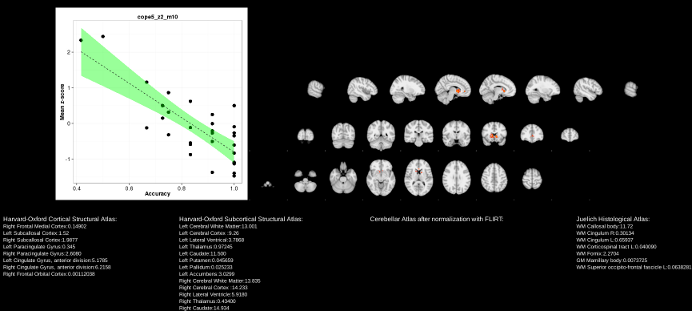
\includegraphics[scale=.6]{images/SSreport.png}
		\caption{Report plotting group FEAT results against behavioral measures.}
                \label{fig:fqresults}
	\end{center}
\end{figure}
